\documentclass[dissertation.tex]{subfiles} 
\begin{document}

\chapter{The Compact Muon Solenoid Experiment}
\label{chap:The Compact Muon Solenoid Experiment}

%keep repeating references to the detector paper?
\textcolor{red}{\textbf{Keep repeating references to the detector paper?}}

The Compact Muon Solenoid (CMS) detector sits at point 5 of the LHC ring, diametrically opposite the ATLAS detector at point 1.  It is a 4$\pi$ hermetic general purpose detector, meaning that it has the capability to detect charged and neutral hadrons, photons, electrons, muons, taus, neutrinos, and non-Standard-Model particles predicted to escape the detector with good efficiency over a large range of rapidity.  Its main distinguishing feature is a superconducting solenoid that provides a 3.8T magnetic field parallel to the beam line.  This strong magnetic field allows precise determination of the momentum and charge of muons and electrons up to a momentum of $\sim$1 TeV.

The origin of the CMS coordinate system is at the nominal interaction point.  The $y$-axis points skyward, the $x$-axis points towards the center of the LHC ring, and the $z$-axis points counterclockwise along the LHC ring.  $r$ denotes radial distances from the beam line, $\phi$ is the azimuthal angle measured with respect to the positive $x$-axis, and $\theta$ is the polar angle measured with respect to the positive $z$-axis.  The \textit{pseudorapidity} $\eta$ is defined as $\eta = -\ln\tan(\theta/2)$, and is a good approximation to rapidity $y = (1/2)\ln((E + p_{z}c)/(E - p_{z}c))$ for relativistic particles.  The transverse momentum and energy ($p_{T}$ and $E_{T}$) of a particle are defined as $p_{T} = p\cos\phi$ and $E_{T} = E\cos\phi$, where $p$ and $E$ are the magnitude of the particle's momentum vector and the particle's total energy, respectively.  A depiction of the CMS coordinate system is shown in Figure~\ref{fig:CMS_coordinate_system}.

\begin{figure}
	\centering
	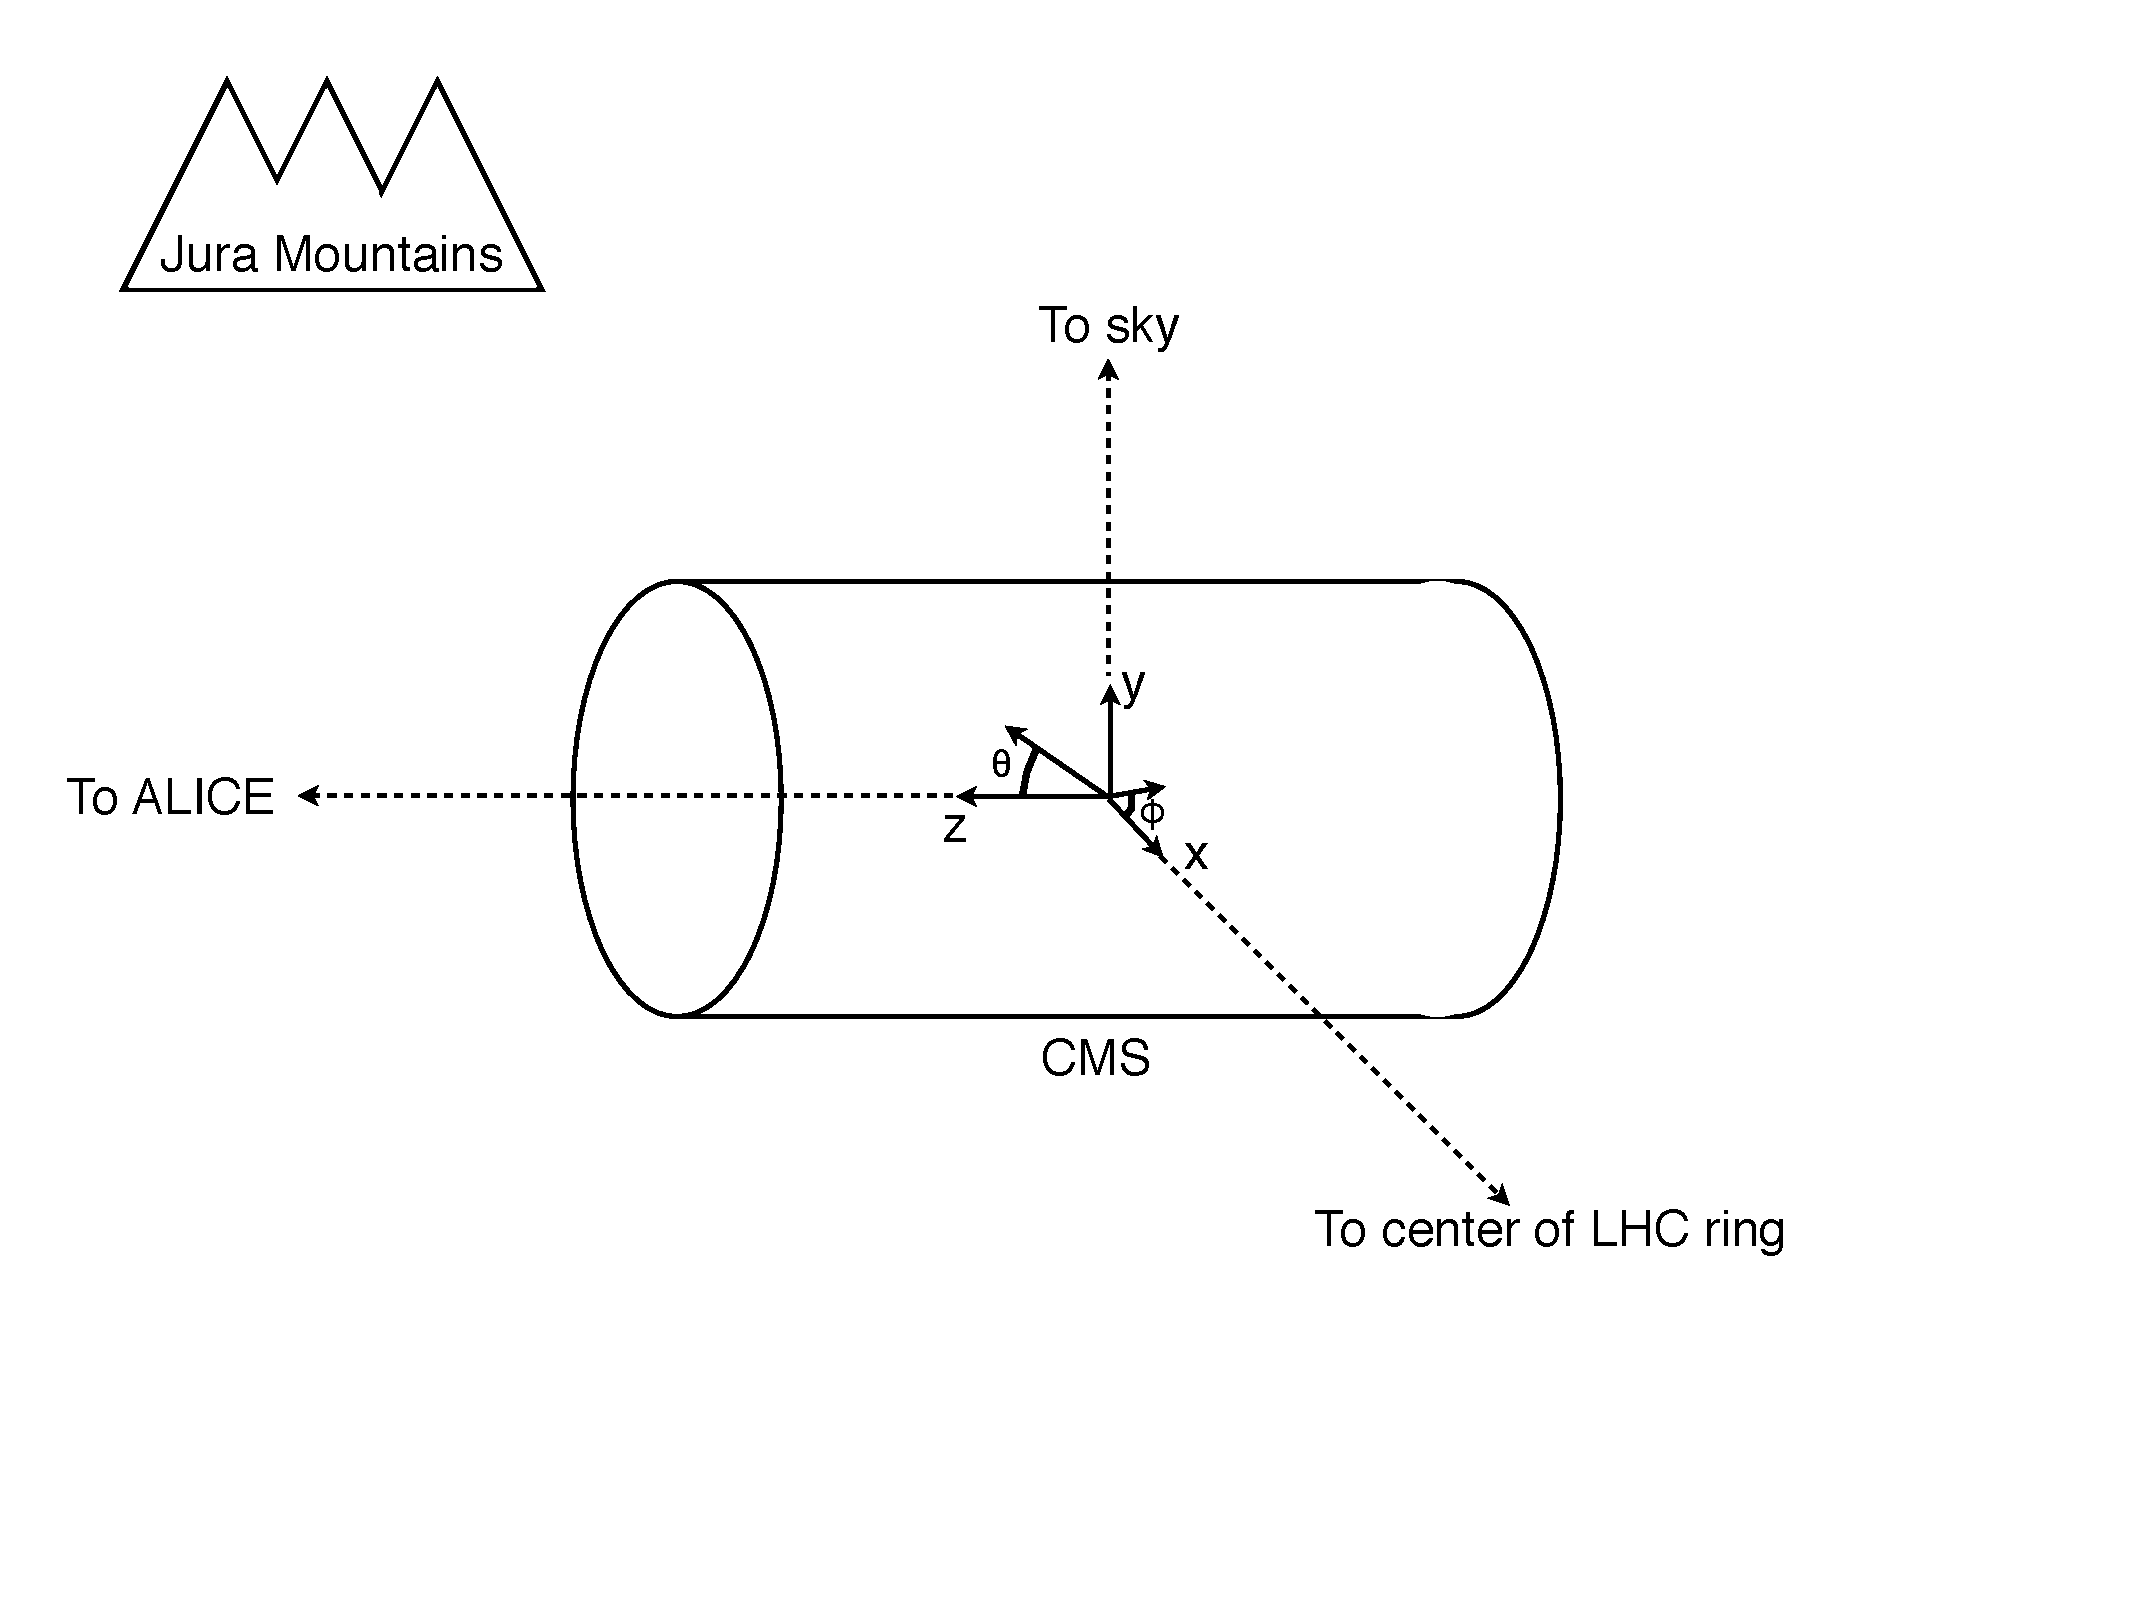
\includegraphics[scale=0.5]{CMS_coordinate_system}
	\caption{CMS coordinate system.}
	\label{fig:CMS_coordinate_system}
\end{figure}

The CMS sub-detectors are arranged in concentric cylindrical layers, plus ``endcaps," around the beam line, as shown in Figure~\ref{fig:CMS_cutaway}.  Closest to the beam line are three layers of silicon pixel detectors, with the innermost at radius 4.4 cm and outermost at radius 10.2 cm \cite{CMS_detector_paper}.  Including the pixel endcaps, the total pixel coverage extends to $\eta$ = 2.5 \cite{CMS_detector_paper}.  The pixel detector plays in important role in determining the proton-proton interaction position (\textit{beam spot}) and the impact parameters of charged particle trajectories, and is critical for the measurement of decay positions some distance from the beam spot (\textit{displaced vertices}), such as those due to the showering and hadronization of a $b$ quark.

\begin{figure}
	\centering
	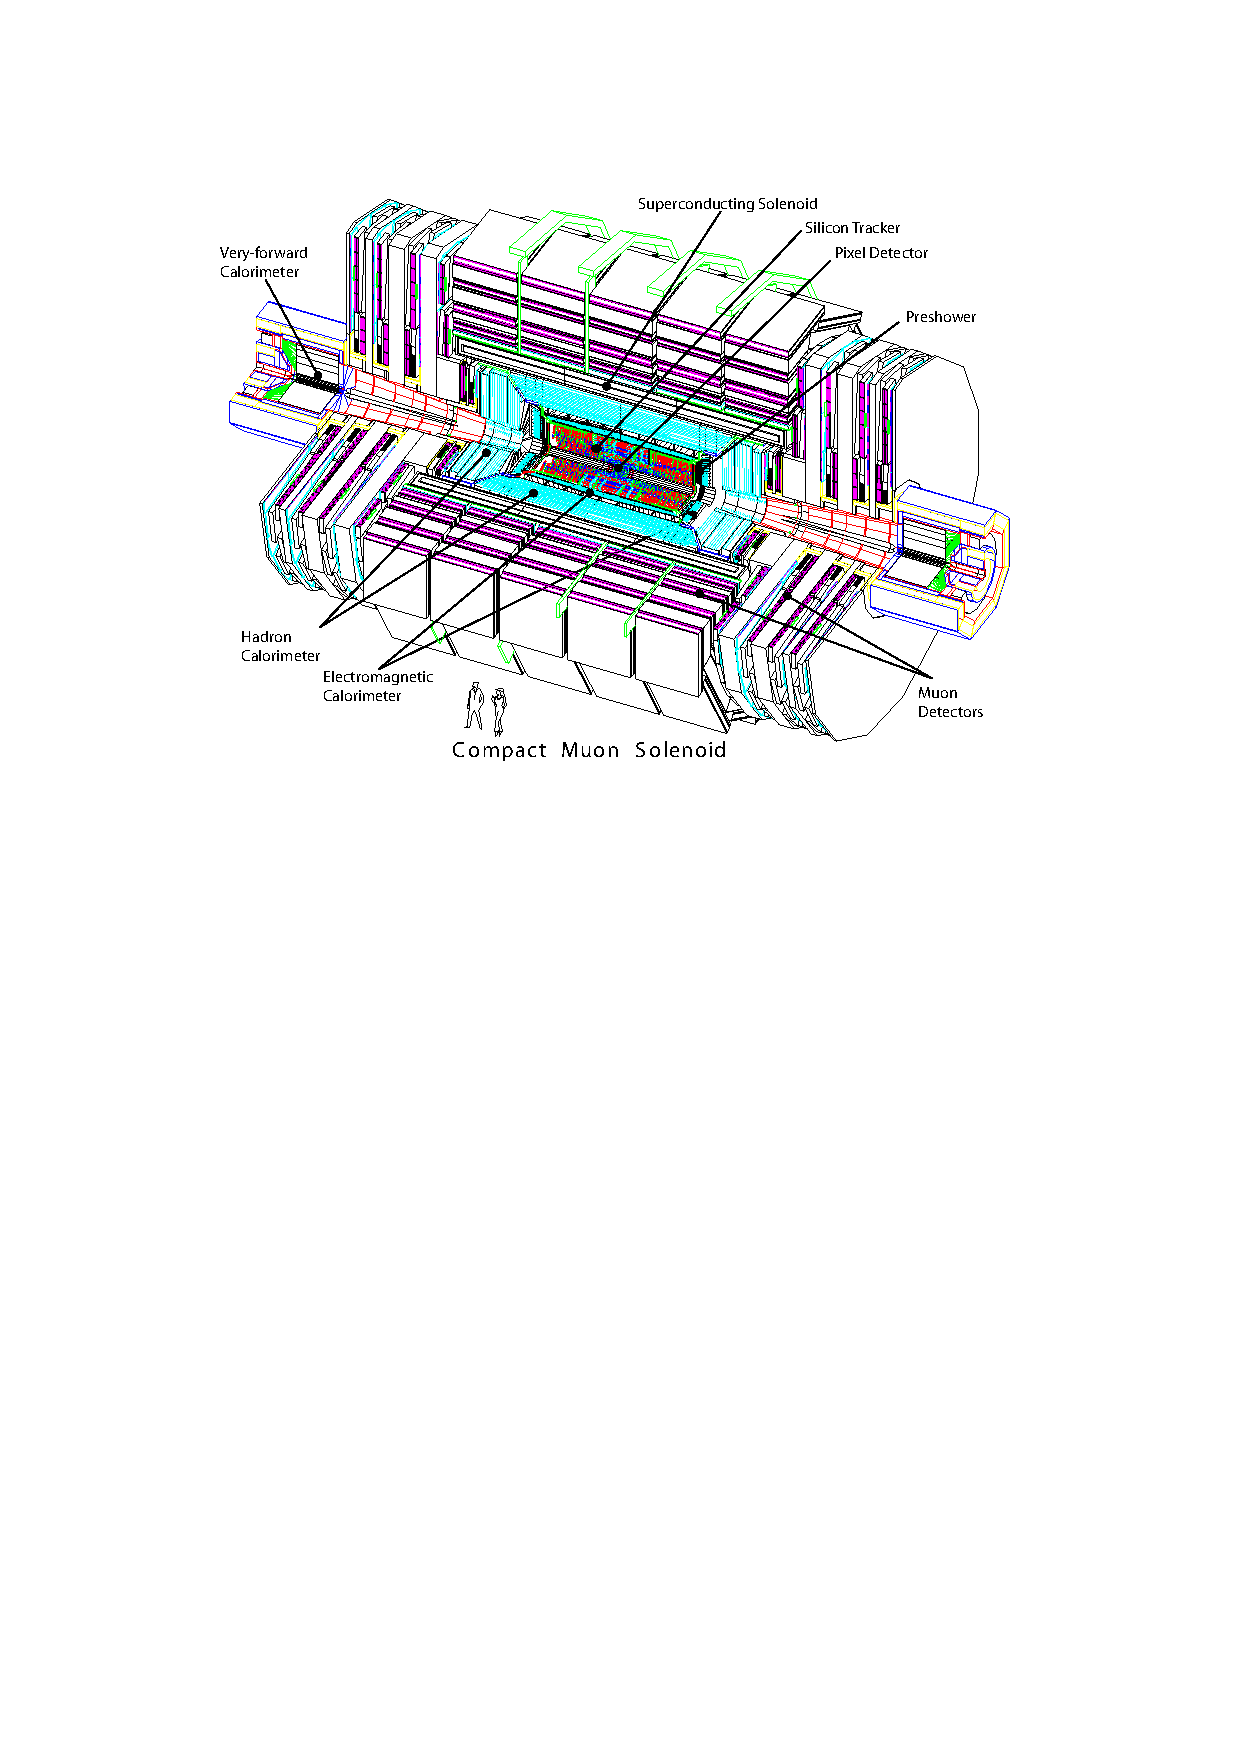
\includegraphics[scale=1.0]{CMS_cutaway}
	\caption{Cutaway view of CMS.  Reprinted from Fig. 1.1 of ref. \cite{CMS_detector_paper}.}
	\label{fig:CMS_cutaway}
\end{figure}

The 10 next layers of CMS are comprised of silicon microstrip detectors, with the outermost layer at a radius of 1.3 m from the beam line \cite{CMS_detector_paper}.  As for the pixel detectors, the silicon strip endcaps extecnd tracking coverage to $\eta$ = 2.5.  The silicon microstrip layers are the workhorse of the CMS tracking system, and provide excellent charged particle momentum resolution and track finding efficiency.

Outside the tracking detectors are the calorimeters, starting with the single-layer lead tungstate crystal electromagnetic calorimeter at a radius of 1.3 m from the beam line (location of crystal front faces) \cite{CMS_detector_paper}.  Each crystal is 23 cm long, corresponding to 25.8 radiation lengths ($\mbox{X}_{0}$).  The crystal dimensions are such that most of one electromagnetic shower, and no more, can be contained in a single crystal, leading to excellent energy resolution for photons and electrons.  The electromagnetic calorimeter radial and endcap layers cover a pseudorapidity range up to 3.0.  A lead/silicon sampling calorimeter sits in front of the crystal endcaps to provide better rejection of neutral pions.

The last layer of calorimetry inside the solenoid is the brass/scintillator sampling hadronic calorimeter, which has a radial extent from 1.77-2.95 m \cite{CMS_detector_paper}.  The hadronic barrel and endcap calorimeters cover up to $|\eta|$ = 3.0, while the iron/quartz-fiber forward hadronic calorimeter covers the region $3.0 \leq |\eta| \leq 5.2$. \footnote{The Centauro and Strange Object Research (CASTOR) and Zero Degree Calorimeter (ZDC) detectors provide additional calorimetry beyond $|\eta| = 5.2$.  However, they are mainly used in the heavy ion and diffractive physics programs of CMS, and play no role in the detection of heavy SUSY particles.  Therefore, they will not be discussed here.}  There is one more layer of hadronic calorimetry outside the solenoid in $|\eta| < 1.3$ which, together with the layers inside the solenoid, provides approximately 12 hadronic interaction lengths of instrumented absorber.  Because of its large $|\eta|$ coverage and depth, the hadronic calorimeter provides good missing transverse energy resolution and accurate measurements of high energy jets.

The iron return yoke of the solenoidal magnetic field is interleaved with muon detectors from 4.1-7.4 m in $r$ and 6.6-10.6 m in $z$, providing muon detection up to $|\eta| = 2.4$ \cite{CMS_detector_paper}.  In the barrel region of $|\eta| < 1.2$, drift tubes are used to read out the muon tracks, while in the endcaps cathode strip chambers are used.  Due to their speed, resistive plate chambers are used throughout the muon system to provide an independent trigger and timing measurement.  Combining the tracker and muon system hits, the momenta and charge of muons up to $p_{T} = 1$ TeV can be precisely reconstructed.

A longitudinal quarter cross-sectional view of CMS is shown in Figure~\ref{fig:CMS_longitudinal_xsec}.  The remainder of this chapter is devoted to explaining the CMS subdetectors and readout systems.  Section~\ref{sec:The Detectors and Their Operating Principles} describes the subdetector technologies and performance benchmarks, while Section~\ref{sec:Triggering, Data Acquisition, and Data Transfer} details the CMS trigger and data acquisition systems and framework for promptly reconstructing and transferring data worldwide.  For a thorough description of CMS, see ref. \cite{CMS_detector_paper}, from which much of the information in the section was culled.

\begin{figure}
	\centering
	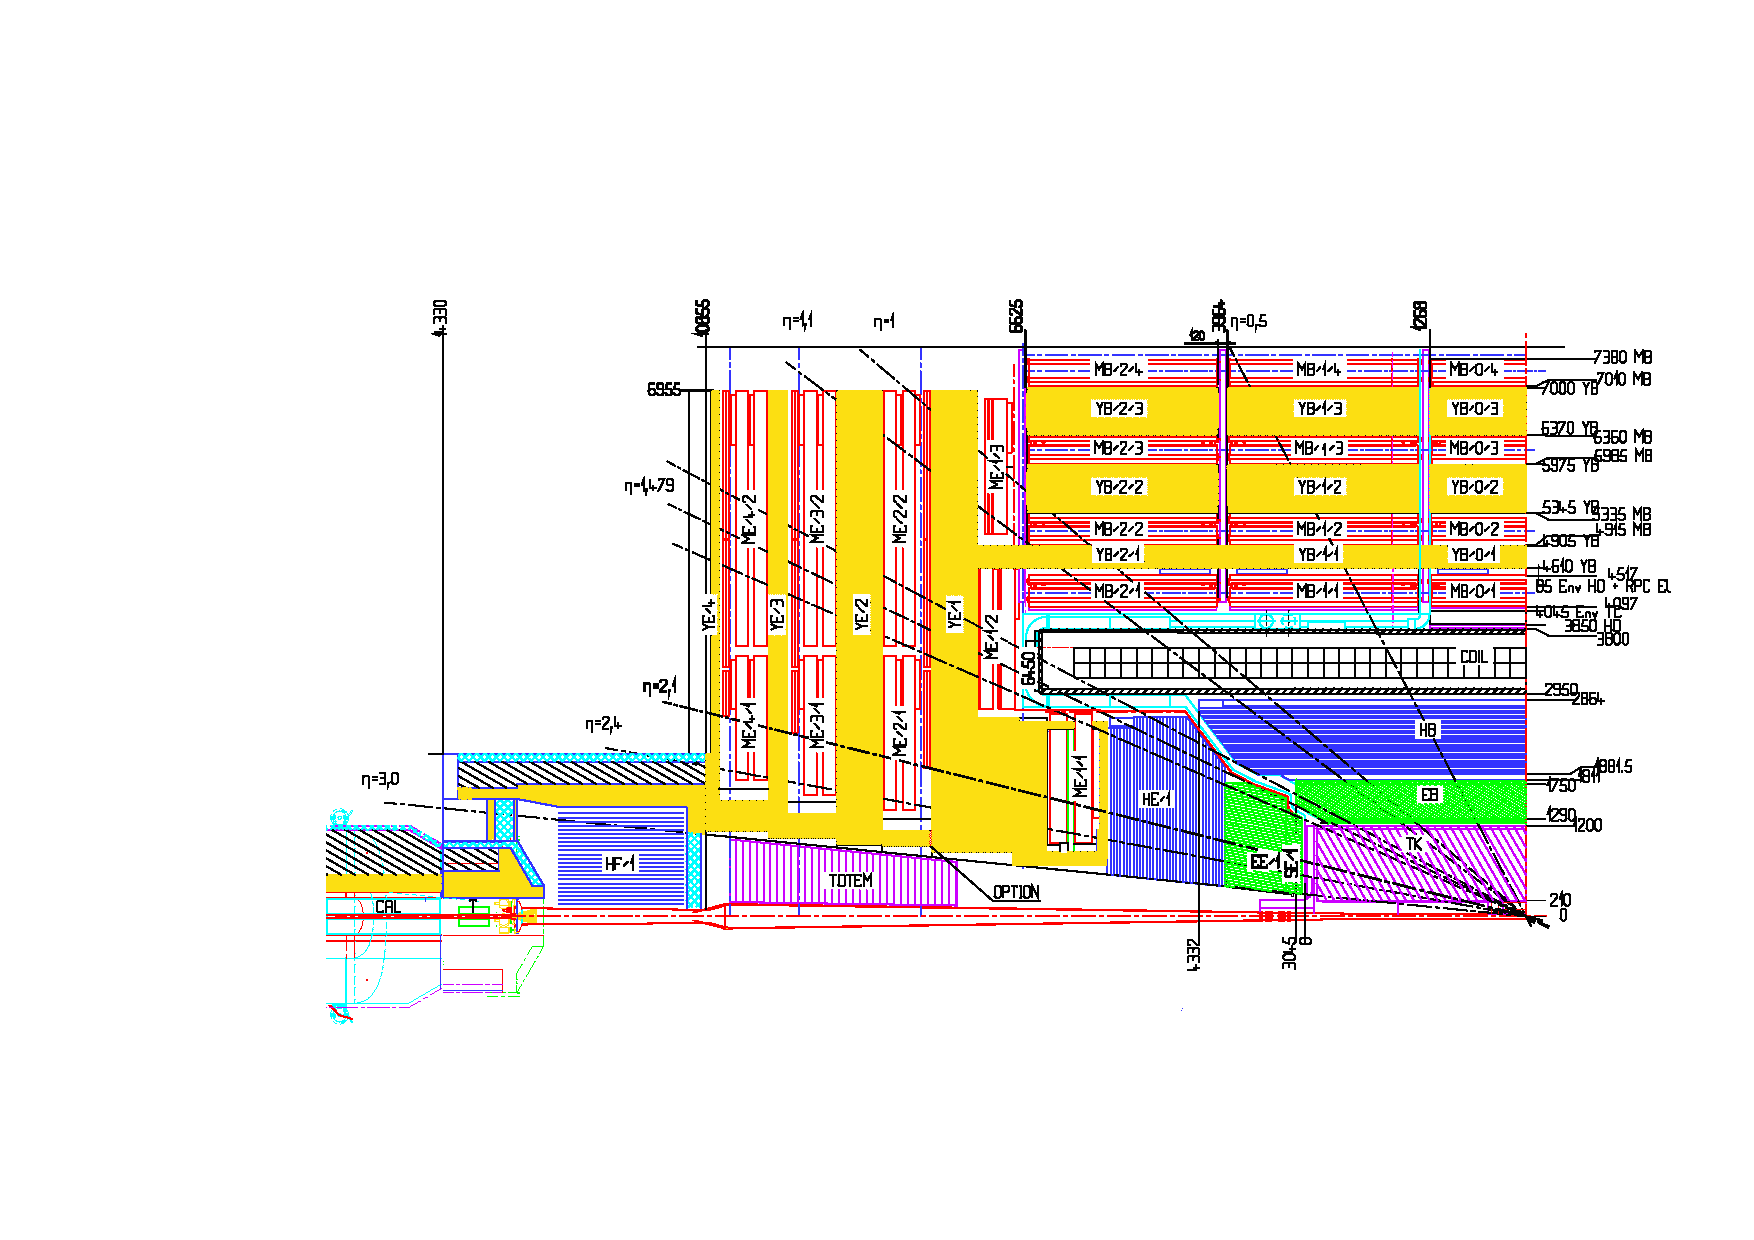
\includegraphics[scale=0.5]{CMS_longitudinal_xsec}
	\caption{Longitudinal quarter cross-sectional view of CMS.  The nominal interaction point is at the lower right-hand corner of the drawing.  The tracker is shown in purple diagonal hashing, the electromagnetic calorimeter in green, the hadronic calorimeter in blue, and the muon stations in red.  The solenoid is shown in black and white and labeled \texttt{COIL}, and the magnet return yoke is shown in yellow.  Radial and longitudinal distances are measured in millimeters.  Reprinted from Fig. CP 1 of ref. \cite{CMS_TDR}.}
	\label{fig:CMS_longitudinal_xsec}
\end{figure}

\section{The Detectors and Their Operating Principles}
\label{sec:The Detectors and Their Operating Principles}

%layout of the detector (names of the sub-parts, technologies used)
%explanation of how the technology works and short motivation for choosing it
%short explanation of the readout
%if the detector triggers, explanation of the trigger primitive generation
%performance benchmarks

\subsection{Tracking System}
\label{sec:Tracking System}

Given the LHC design instantaneous luminosity, efficient reconstruction of charged particle tracks from transverse momenta of 1 GeV up to 1 TeV can only be achieved with a low occupancy tracker.  For $r < 10$ cm, the hit rate density is highest, leading to the choice of $100\mbox{ }\mu\mbox{m} \times 150\mbox{ }\mu\mbox{m}$ silicon pixel sensors for hit detection.  For $20\mbox{ cm }< r < 110\mbox{ cm}$, the lower hit rate allows the use of silicon strips, with length along $z$ of order centimeters and length along the $r\cdot\phi$ curve of order hundreds of microns.  This design leads to a pixel hit occupancy of $\sim10^{-4}$/pixel/BX and a strip hit occupancy of $\sim10^{-2}$/pixel/BX, where BX refers to 1 LHC bunch crossing \cite{CMS_detector_paper}.

As radiation dose from hadrons accumulates over the lifetime of the tracker, silicon leakage current through the semiconductor junctions increases, heating up the sensors.  Since the leakage current itself depends on temperature, this can lead to \textit{thermal runaway} that damages the detector.  To avoid this, the tracker must be cooled to approximately $-10^{\circ}$C.  Operating at this temperature, the signal:noise ratio in the silicon sensors is 10:1, and should remain at that level over the 10-year lifetime of the tracker \cite{CMS_detector_paper}.

At its thickest ($|\eta|\sim1.5$), the tracker depth (including services) is $\sim1.8X_{0}$, and the depth falls off to $\sim1X_{0}$ in thinner areas.  Unfortunately, the large mass of the tracker degrades somewhat the performance of the electromagnetic calorimeter behind it, as $\sim50$\% of photons will convert to $e^{+}e^{-}$ pairs in the tracker.

\subsubsection{Pixel Detector}
\label{sec:Pixel Detector}

A longitudinal quarter view of the three barrel pixel (BPix) layers and two forward pixel (FPix) disks is shown in Figure~\ref{fig:pixel_longitudinal_quarter_view}.  There are 768 BPix modules in total.  Each BPix layer is divided into 32 $\phi$-wedges, with eight modules per wedge arranged end-to-end in $z$.  The $\phi$-wedges operate nearly independently in terms of clock and readout.  Each FPix disk consists of 24 $\phi$-wedges, with pie-shaped modules attached to the front and back of the disk, for a total of 192 modules.  The front- and back-side modules of the FPix disks are constructed of different sized \textit{plaquettes}, or multi-pixel sensor chips, such that the gaps in the front-side module are covered by plaquette area in the back-side module and vice versa.  An illustration of the BPix and FPix mechanical layouts is given in Figure~\ref{fig:pixel_mechanics}.

\begin{figure}
	\centering
	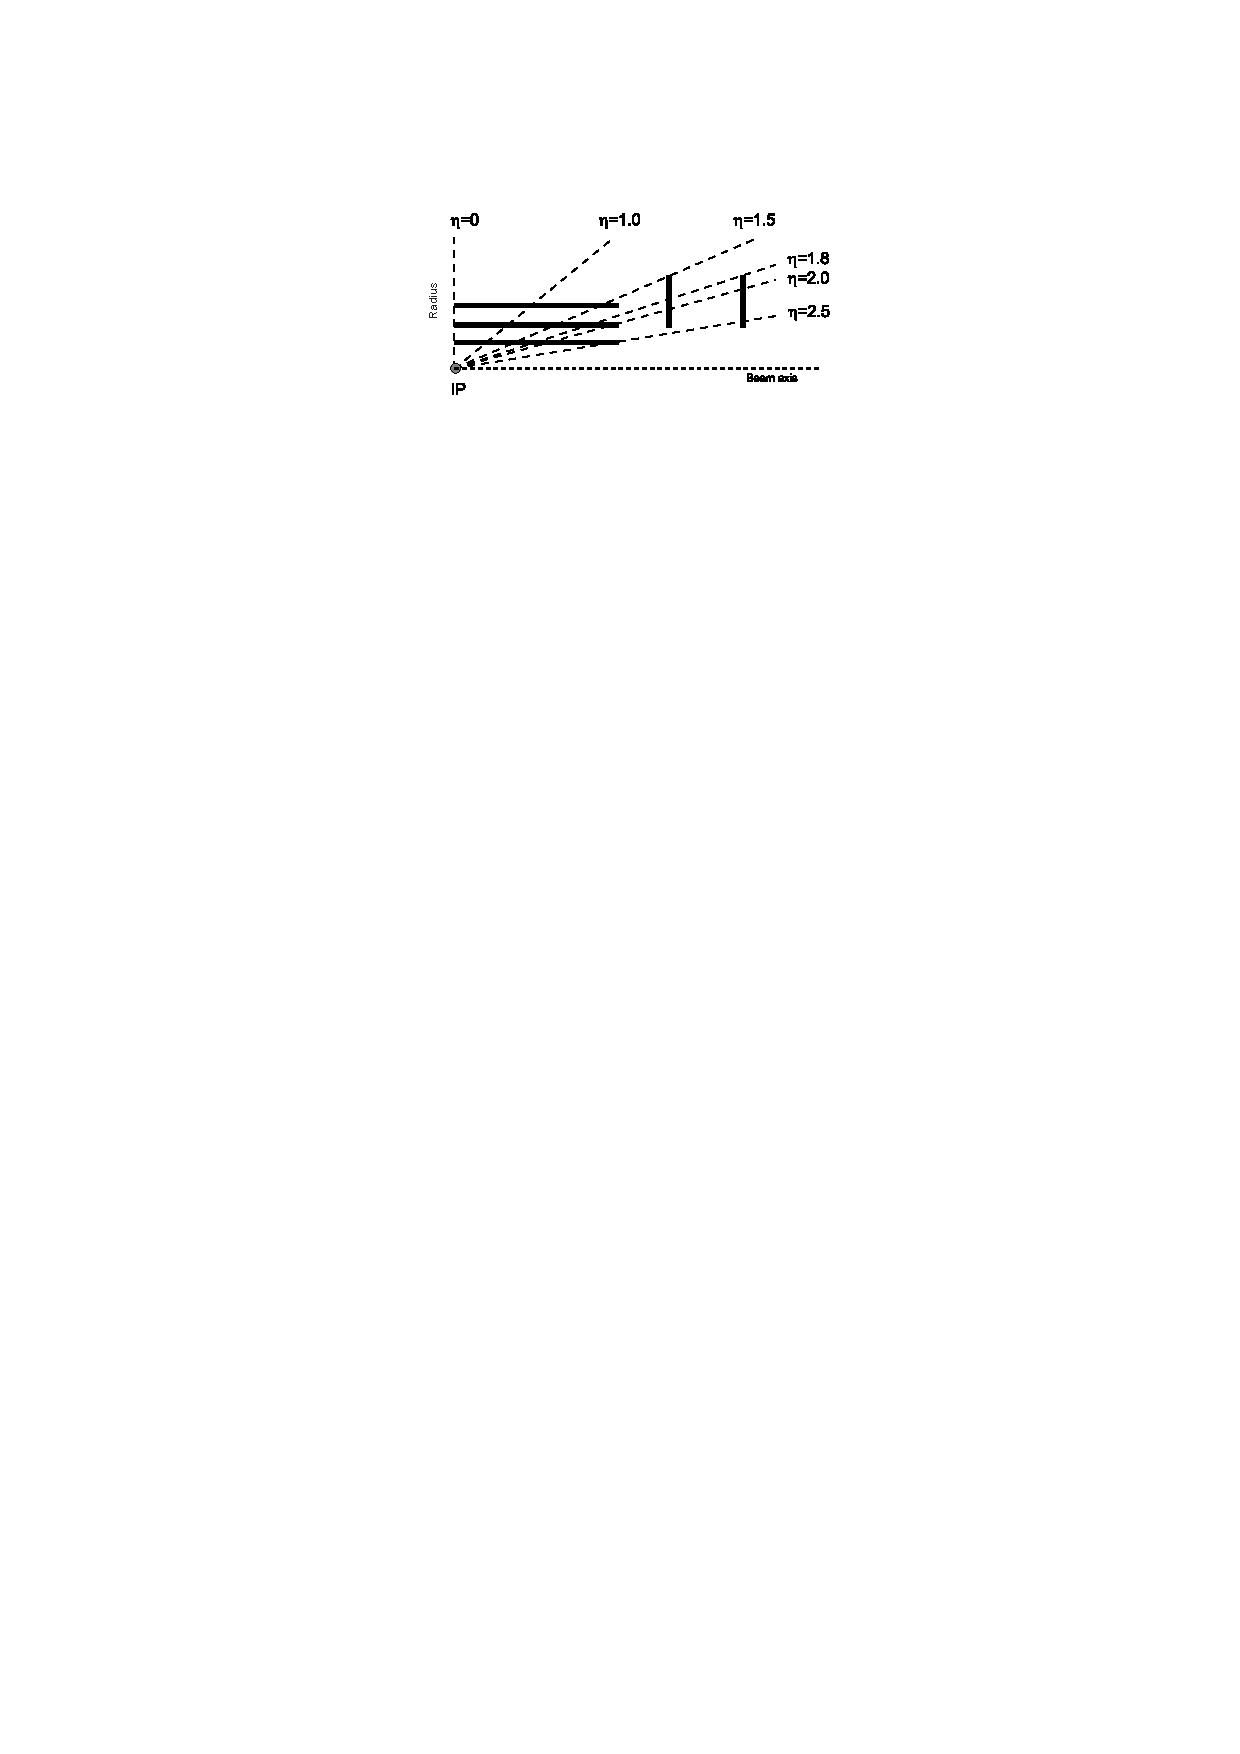
\includegraphics[scale=1.0]{pixel_longitudinal_quarter_view}
	\caption{Longitudinal quarter view of the pixel detector.  Reprinted from Fig. 3.6 of ref. \cite{CMS_detector_paper}.}
	\label{fig:pixel_longitudinal_quarter_view}
\end{figure}

\begin{figure}
	\centering
 	\subfloat[Cutaway view of the barrel pixel layers, showing the three layers and the eight end-to-end modules along $z$.  Reprinted from Fig. 3.11 of ref. \cite{CMS_detector_paper}.]{\label{fig:BPix_mechanics}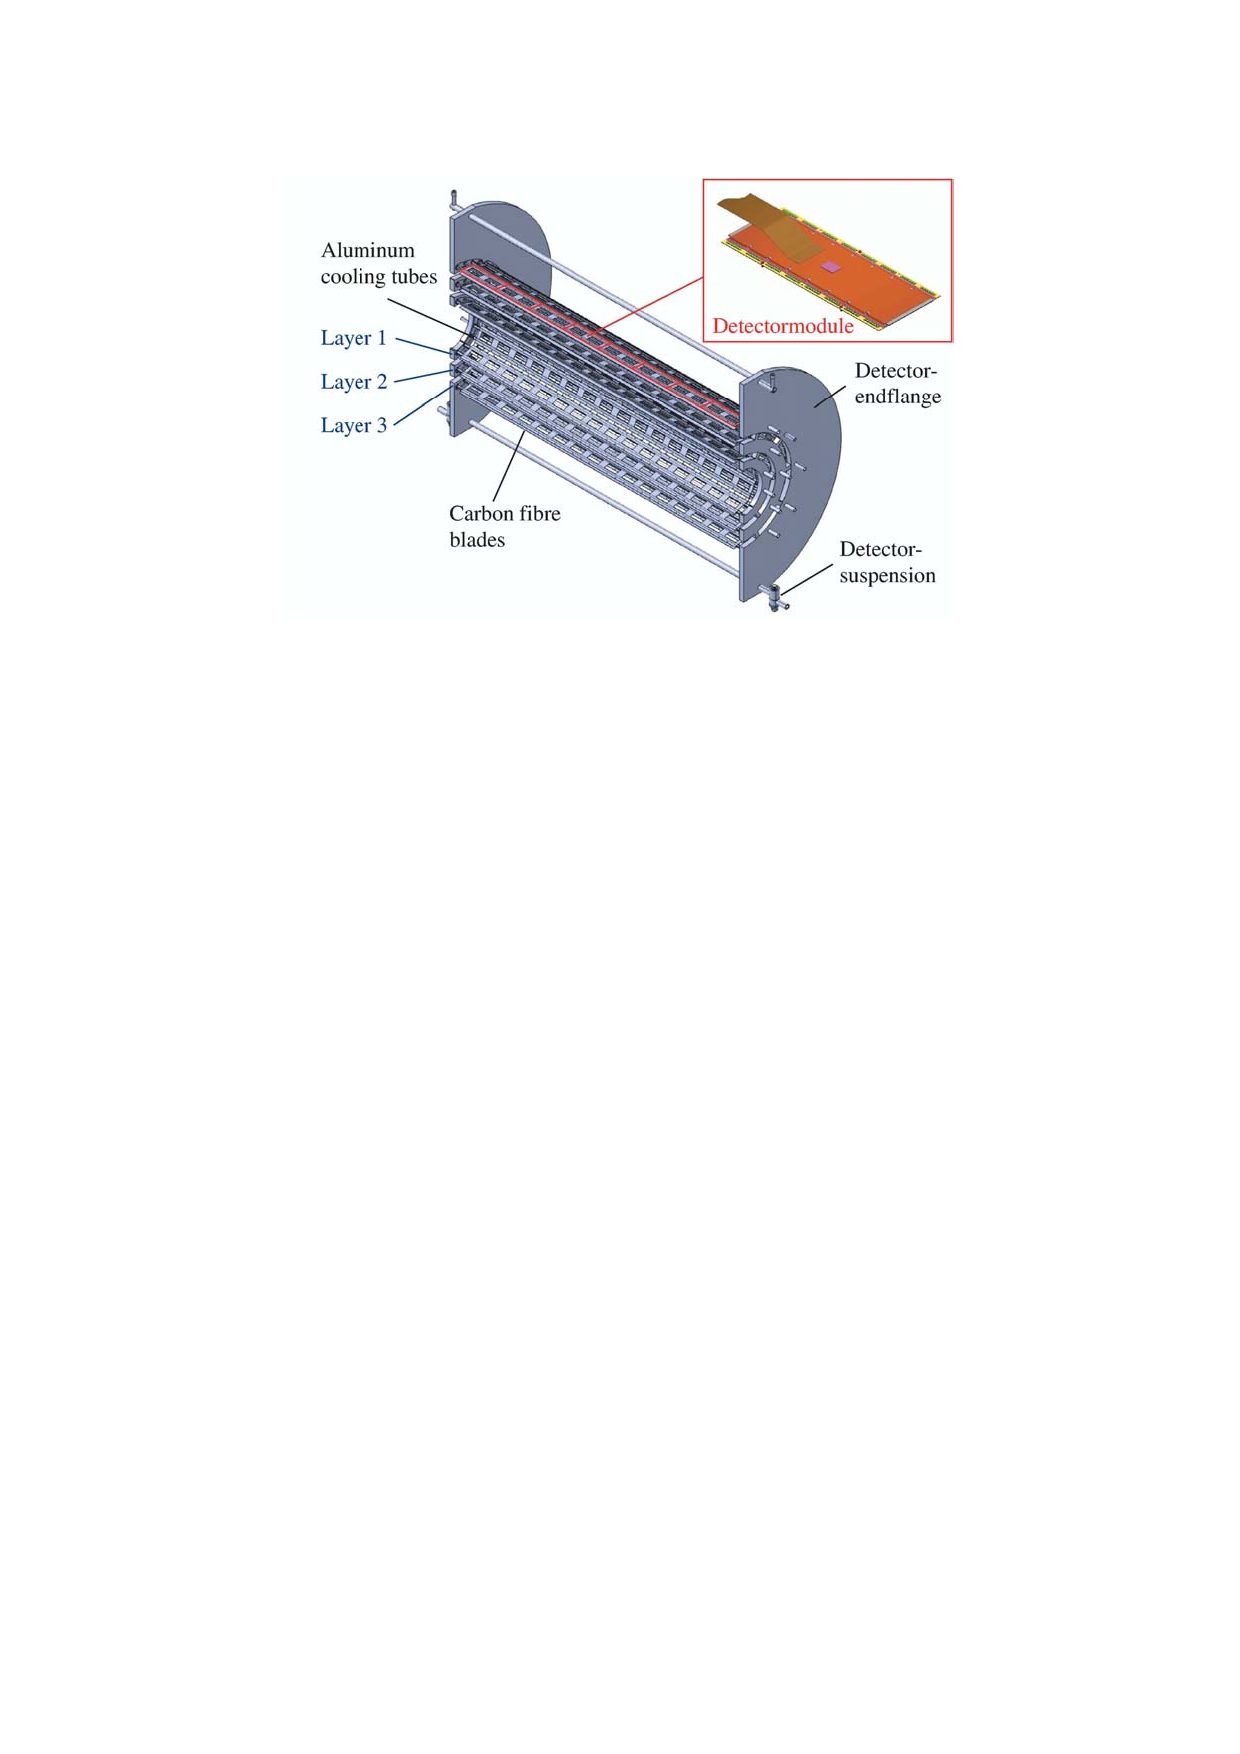
\includegraphics[scale=0.6]{BPix_mechanics}}
	\hspace{1cm}
	\subfloat[Half-disk of the foward pixel detector, showing the 12 pie-shaped module mounts.  Reprinted from Fig. 3.15 of ref. \cite{CMS_detector_paper}.]{\label{fig:FPix_mechanics}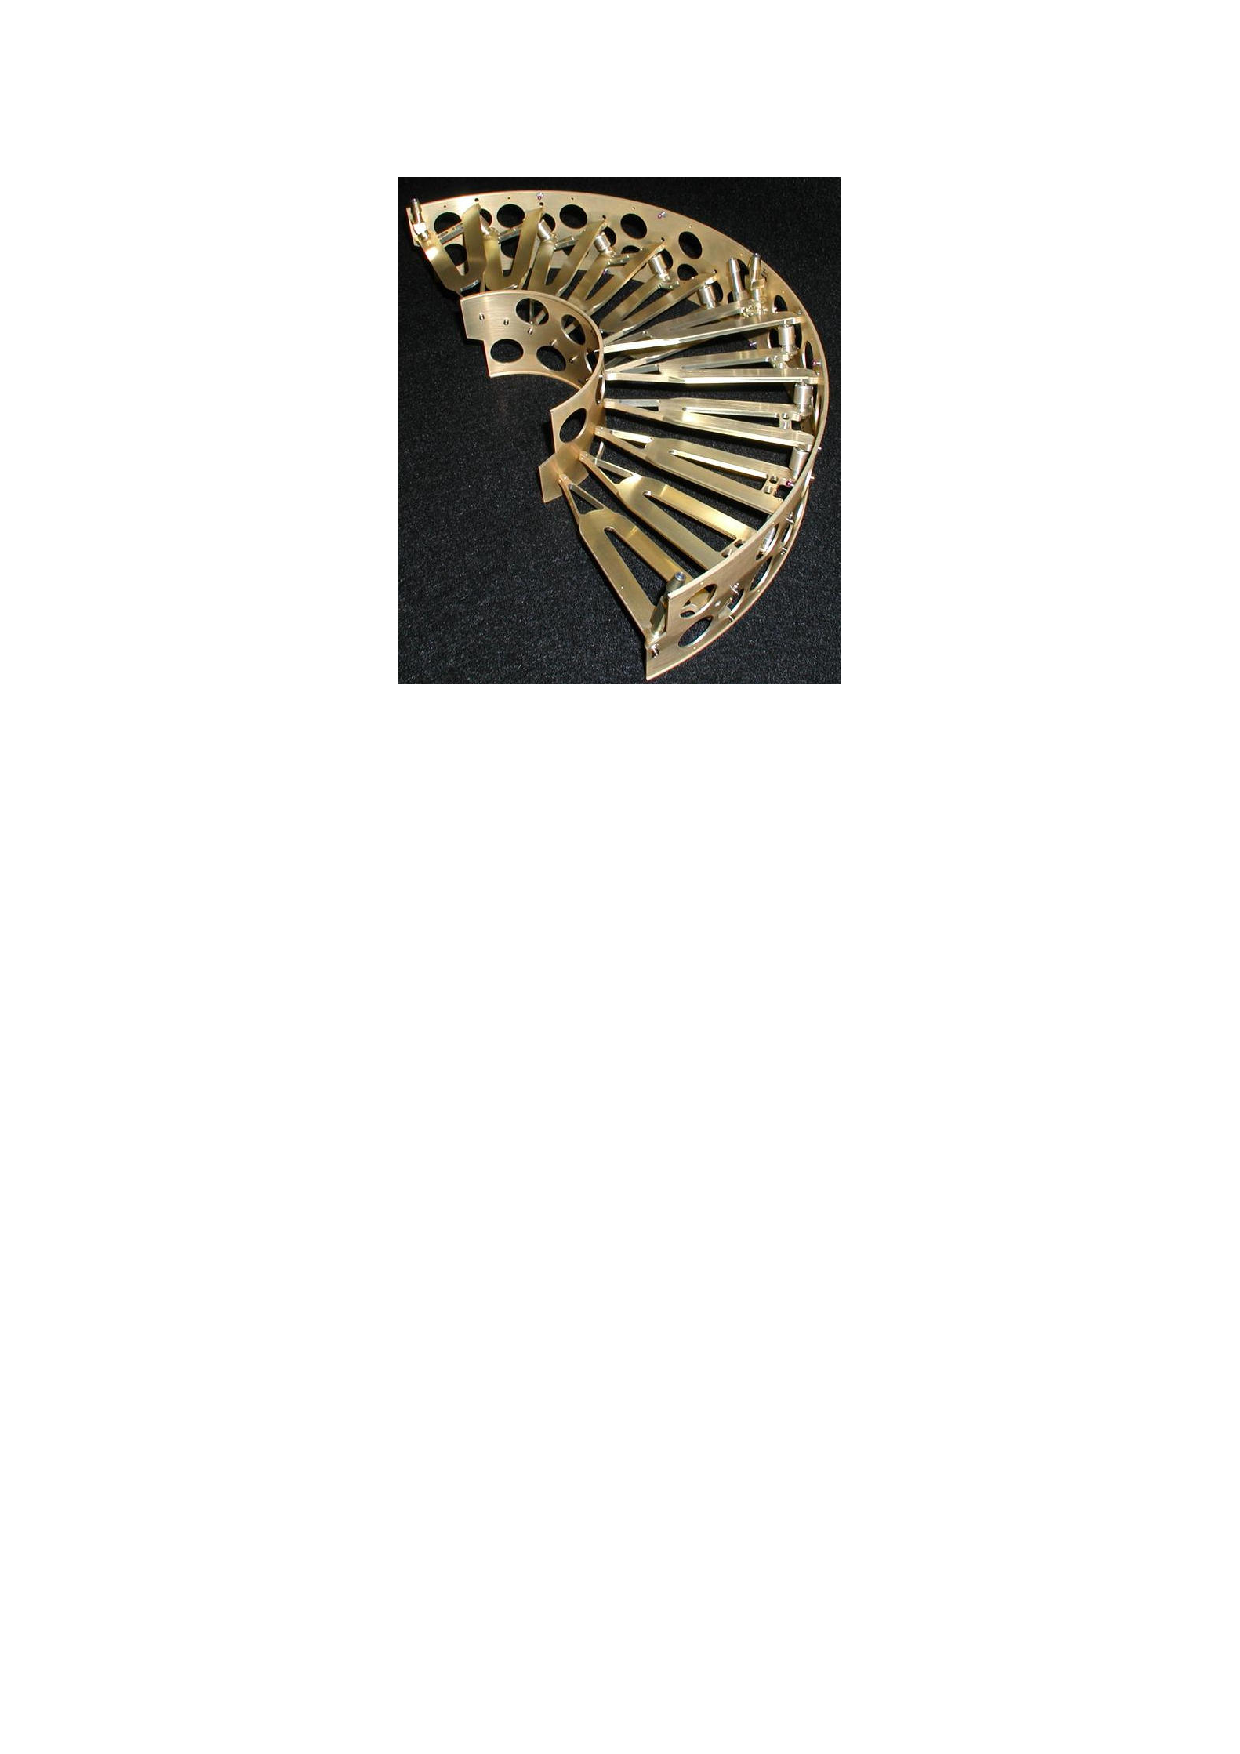
\includegraphics[scale=0.6]{FPix_mechanics}}
	\caption{BPix and FPix mechanical structures.}
	\label{fig:pixel_mechanics}
\end{figure}

%insert reference to BPix Lorentz angle
Since the electric field in the depletion region of the BPix sensors is perpendicular (i.e. pointing along $r$) to the magnetic field of CMS (i.e. pointing along $z$), the charge carriers in the silicon experience a Lorentz drift along $\phi$.  The multi-pixel sensor pitch is such that this causes the charge from one particle hit to be shared among multiple pixels.  Particle hits are reconstructed reading out the analog pixel signal and interpolating between signals in multiple pixels.  This method achieves a 15-20 $\mu\mbox{m}$ spatial resolution, which is comparable to the sensor pitch.  To induce this effect in FPix, the sensor wedges are tilted by the BPix Lorentz angle of $20^{\circ}$ \textcolor{red}{\textbf{(insert reference to BPix Lorentz angle)}} with respect to the $y$-axis.

%sensor technology, bias voltage
%readout system (diagram)
%performance

\subsubsection{Silicon Strip Tracker}
\subsection{Electromagnetic Calorimeter}
\label{sec:Electromagnetic Calorimeter}
%make this big, include EE work
%discuss crystal radiation damage
\subsection{Hadronic Calorimeter}
\subsection{Muon System}
%spend very little time on this

\section{Triggering, Data Acquisition, and Data Transfer}
\label{sec:Triggering, Data Acquisition, and Data Transfer}

\subsection{Level 1 and High Level Trigger Systems}
\label{sec:Level 1 and High Level Trigger Systems}
%talk about trigger primitives for the ECAL especially (there is a reference to this section from the HLT section in ch. 6 when we talk about L1 seeds), SR, etc.
\subsection{Data Acquisition System}
\subsection{Data Processing and Transfer to Computing Centers}
\label{sec:Data Processing and Transfer to Computing Centers}
%define lumi section

Lorum ipsum fuck Republicans.

\end{document}